\documentclass[./\jobname.tex]{subfiles}
\begin{document}
%
% A UML class diagram of the static software structure.
% The classes shall include at least the names of the methods (operations) with parameter and return values.
% Classes with active/reactive behaviour shall be highlighted e.g. using a colour.
% A brief textual description of the classes is only needed if specific properties and/or functionality cannot be understood from the diagram only.
%
\chapter{Statische Software Struktur}
%
In diesem Kapitel wird das statische Softwarekonzept vorgestellt. Für die Erstellung wird \gls{uml} verwendet und mittels Astah\footnote{\url{http://astah.net}} erstellt.
%
\section{Designmodell}
%
In \autoref{fig: OS.pdf} ist die erstellte statische Software Struktur abgebildet. Zentrale Komponente der Architektur stellt die Klasse \enquote{ConveyorBelt} dar. Diese erstellt und verwaltet mittels Statemachine sämtliche für die Anwendung benötigten Objekte.\par
%
Alle aktiven Klassen, inklusive der Klasse Display, werden als eigenständige Tasks ausgeführt.
Die Klassen \enquote{TCPServer}, \enquote{TCPClient}, \enquote{TelnetServer} und \enquote{Keyboard} dienen zur Kommunikation zwischen Förderbändern sowie zwischen Förderband und menschlichem Operator. Das Interface \enquote{ICommunication} stellt sicher, dass Klassen mit bidirektionaler Kommunikation die grundlegenden Methoden implementiert haben müssen.\par
%
Die Klasse \enquote{Controller} beinhaltet den Regler für den Förderbandmotor und die Logik für das Abfahren der Geschwindigkeitsprofile. Der Controller erstellt darüber hinaus ein Objekt vom Typ \enquote{IMotor}, welches mit der Klasse \enquote{Motor} initialisiert wird.\par
%
Die Klasse \enquote{Display} dient zur Visualisierung der aktuellen Zustandsgrößen. Es verwendet die \enquote{Getter} Funktionen der Klassen \enquote{Controller} und \enquote{ConveyorBelt}.
%

%
\begin{figure}[H]
	\centering
	\noindent\adjustbox{max width=\textwidth}{%falls größer als \textwidth, wird das Bild verkleinert
		%trim option's parameter order: left bottom right top
		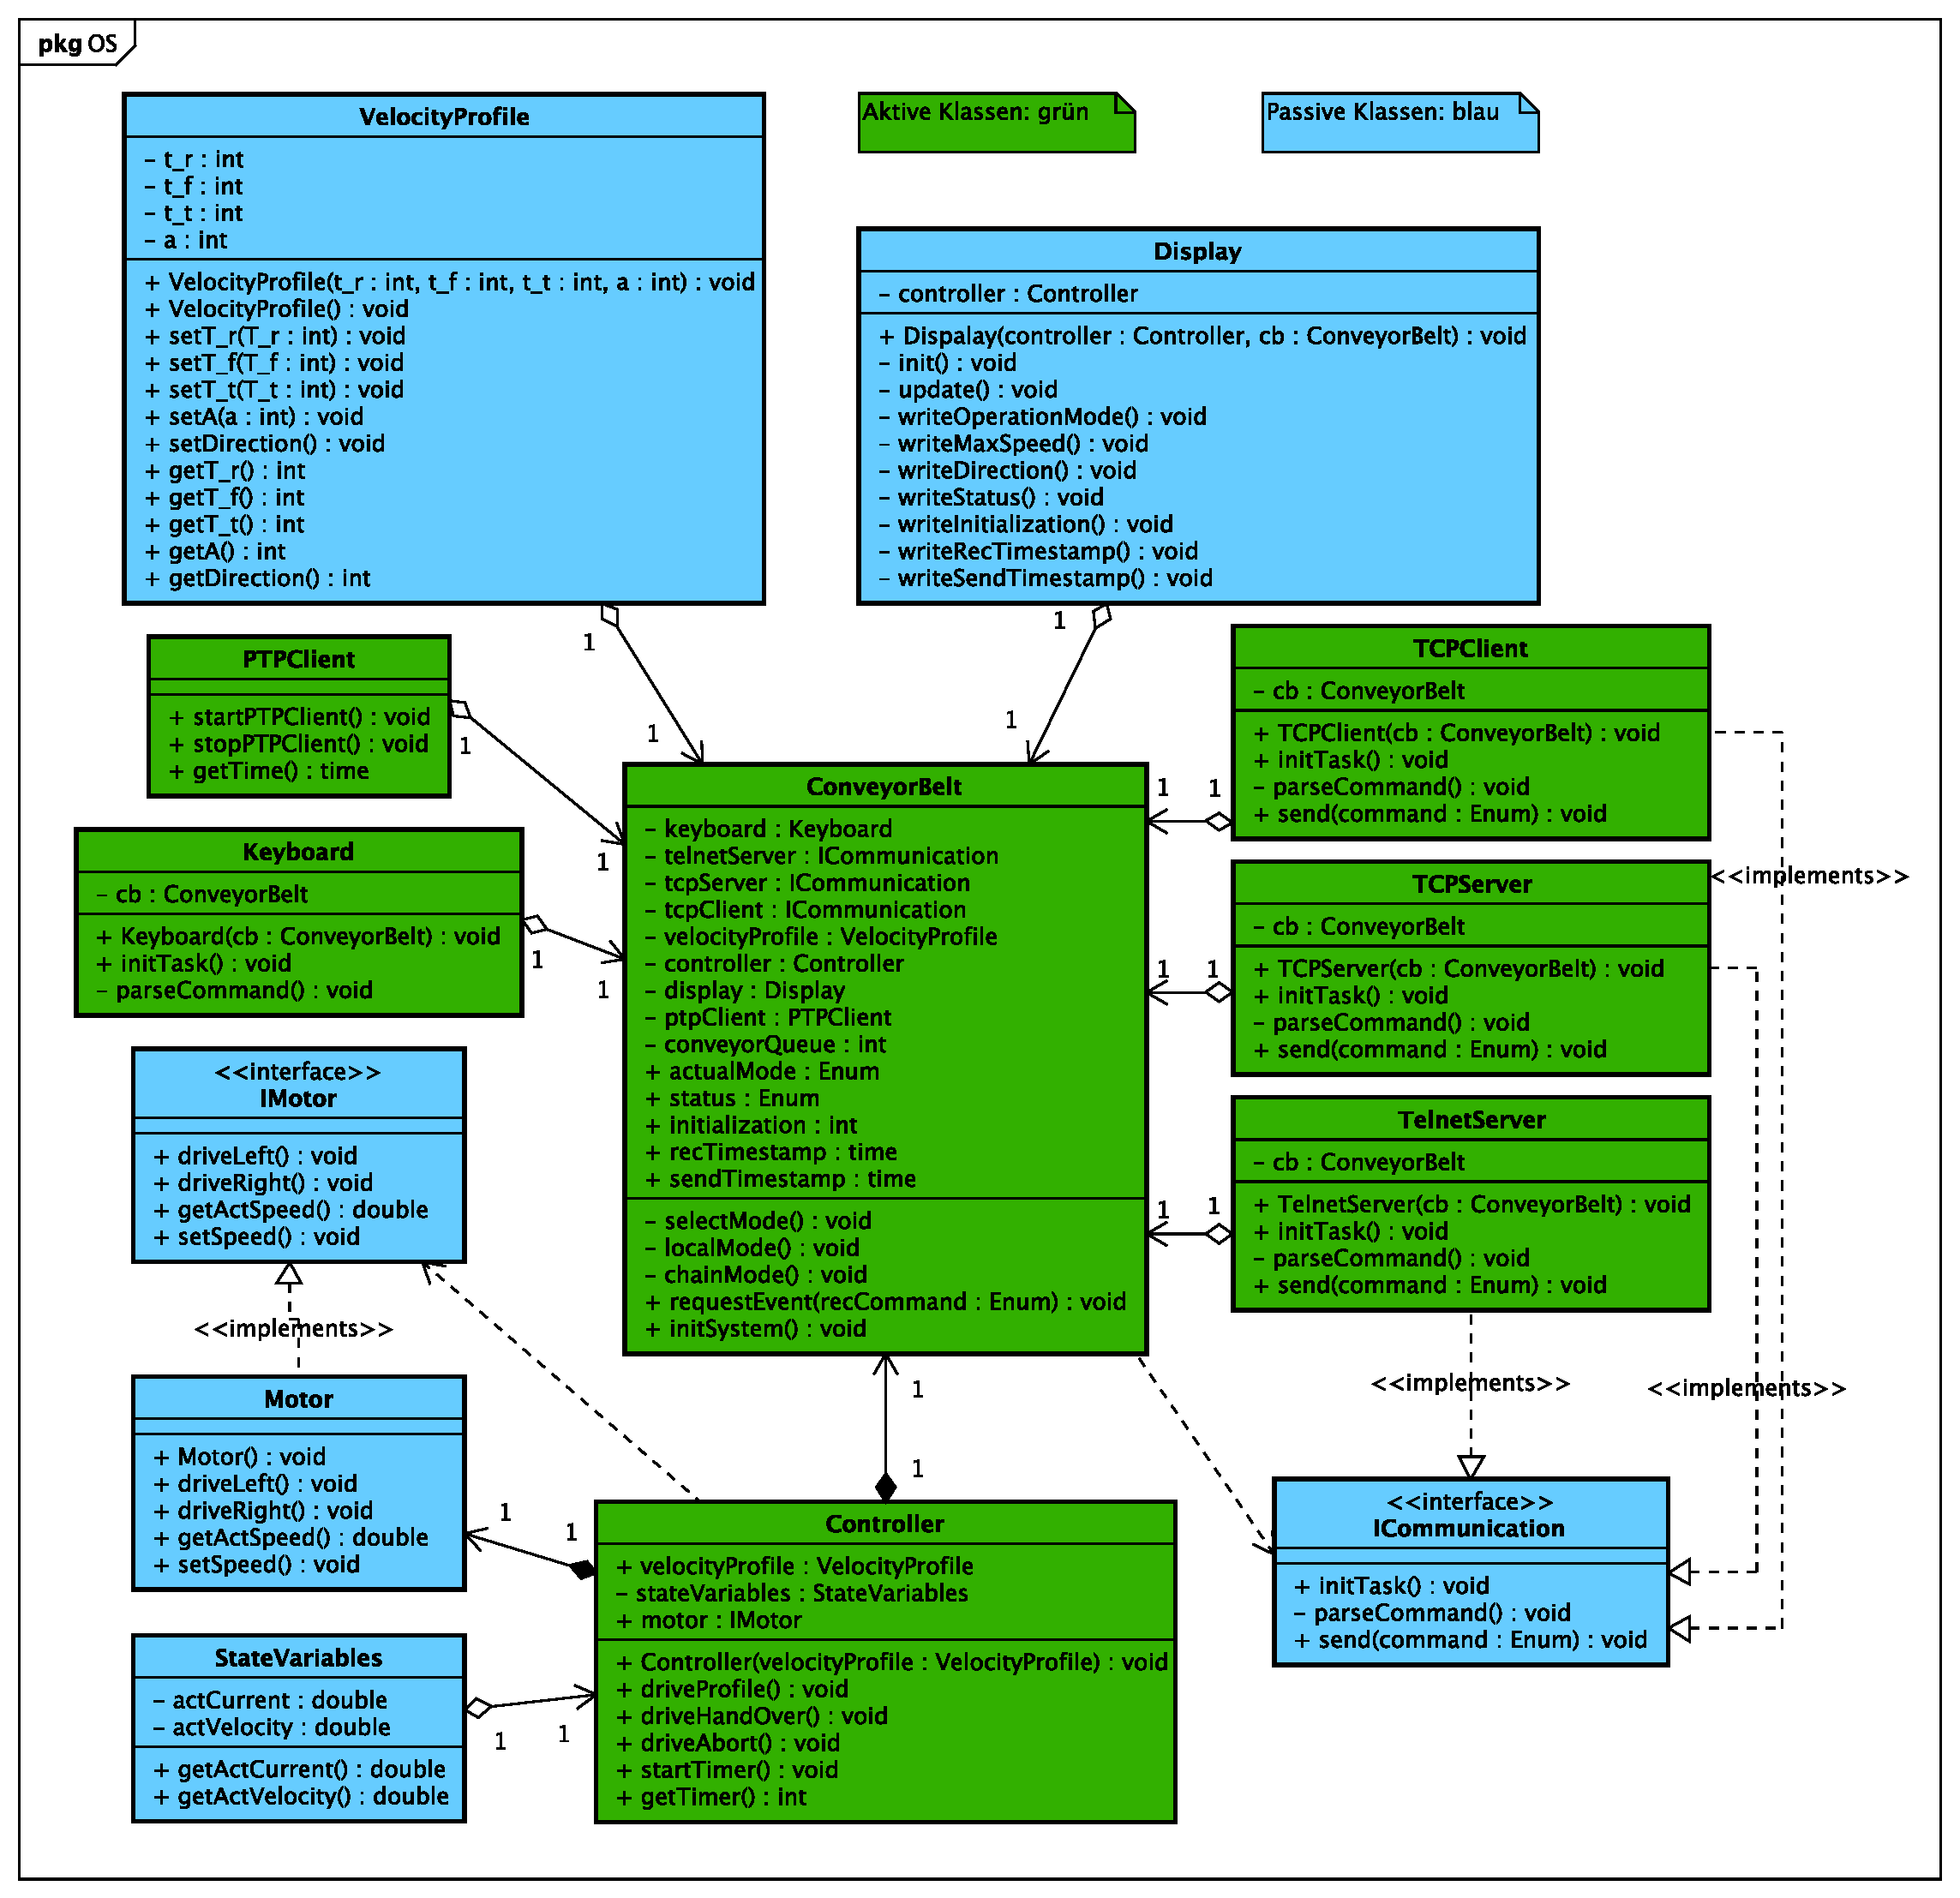
\includegraphics[width=1\textwidth]{./img/2_stat_software_strukt/OS.pdf}
	}
	\unterschrift{Designmodell-Klassendiagramm}{Eigene Ausarbeitung}{}
	\label{fig: OS.pdf}
\end{figure}
%
\section{Implementierungsmodell}
%
In diesem Abschnitt werden die Unterschiede und wichtige Implementierungsdetails im Vergleich zum Designmodell erläutert.
In \autoref{fig: ClassDiagram_implementation.pdf} ist das implementierte Klassendiagramm dargestellt. Im Vergleich zum Designmodell in \autoref{fig: OS.pdf} wird die Klasse \enquote{ConveyorBelt} jetzt \enquote{SystemManager} genannt.\par
%
Weiters wird der \enquote{Parser} jetzt über eine eigene Klasse implementiert. Das bedeutet die Kommunikationsschnittstellen erstellen ein Objekt von der Klasse \enquote{Parser} über welches sie bei Empfang einer Eingabe über die Methode \enquote{parseCommand()} zugreifen. Dabei stellt der \enquote{Parser} fest, ob das Kommando für die Schnittstelle zulässig ist und gibt einen \enquote{Enum} mit dem zulässigen Kommando zurück. Die jeweilige Kommunikationsschnittstelle reicht in weiterer Folge über eine Instanz von der Klasse \enquote{SystemManager} über den Methodenaufruf \enquote{requestEvent} den erhaltenen \enquote{Enum} weiter. Je nach \enquote{Enum} wird dann ein Event der Klasse \enquote{StateMachine} gesendet, welches das Verhaltensmodell von \autoref{sec: Implementierungsmodelle} implementiert.\par
%
Ein weiters Implementierungsdetail betrifft die Vermischung von C und C++ Code in Klassen die Tasks spawnen. Dabei wird über eine \enquote{Task init} Methode der Task gespawnt. Es wird ein \enquote{WorkerTask} von der Klasse erstellt, in dem von der eigenen Klasse ein Objekt erstellt und die \enquote{run} Methode ausgeführt wird. Wird diese Vorgehensweise implementiert, können Instanzen von anderen C++ Klassen im \enquote{WorkerTask} verwendet werden, ansonsten müsste über globale Variablen der Informationsaustausch erfolgen, dadurch könnten nicht autorisierte Klassen auf Variablen zugreifen, das wird mit diesem Modell verhindert.\par
%
Im Designmodell ist eine Klasse für den \enquote{TCPClient} und eine für den \enquote{TelnetServer} vorgesehen. Da beide Klassen den selben Typ von Schnittstelle implementieren, wird im Implementierungsmodell für diese jeweils eine Instanz von der Klasse \enquote{TcpServer} erstellt. Das kann auch dadurch realisiert werden, weil der \enquote{Parser} im Implementierungsmodell in einer eigenen Klasse ausgelagert wird und dieser je nach Instanz zwischen TCPServer und TelnetServer Verbindung unterscheidet und die zulässigen Kommandos als \enquote{Enum} liefert.\par
%
Das Interface \enquote{IMotor} und die Klasse \enquote{StateVariables} wurden im Implementierungsmodell nicht umgesetzt.\par
%
Die Klasse \enquote{Controller} beinhaltet das Reglermodell, welches mit Hilfe von Simulink modelliert und exportiert wurde. Das Modell wurde in C++ Code adaptiert. Die Taktfrequenz wird mit einem Softwarewatchdog mit jener des SystemManagers synchronisiert. Das Verhalten des Geschwindigkeitsprofils vom Motor ist ebenfalls in dieser Klasse implementiert.\par
%
Weiters wurde die Klasse \enquote{UdpClient} hinzugefügt. Diese wird für den Nachrichtenaustausch zwischen \acrshort{ptp}-Client und \acrshort{ptp}-Server verwendet.\par
%
Um die Drehzahl zu ermitteln, wurde eine \enquote{Encoder} Klasse erstellt. Diese implementiert jeweils zwei unterschiedliche Arten der Drehzahlmessung.
\begin{description}
	\item[Counter Zeitdifferenz] Hier wird die Zeitdifferenz der Änderung zum letzten Encoderimpuls ermittelt. Diese Implementierung unterstützt die Ausgabe von Rohdaten, gemittelten Daten und mittels Kalman 1D gefilterte Daten.
	\item[Counter gemittelte Werte] Hier werden die Encoderompulse gezählt und über die verstrichene Zeit vom letzten Aufruf der Methode, kann die Drehzahl ermittelt werden.
\end{description}
%
\begin{figure}[H]
	\centering
	\noindent\adjustbox{max width=\textwidth}{%falls größer als \textwidth, wird das Bild verkleinert
		%trim option's parameter order: left bottom right top
		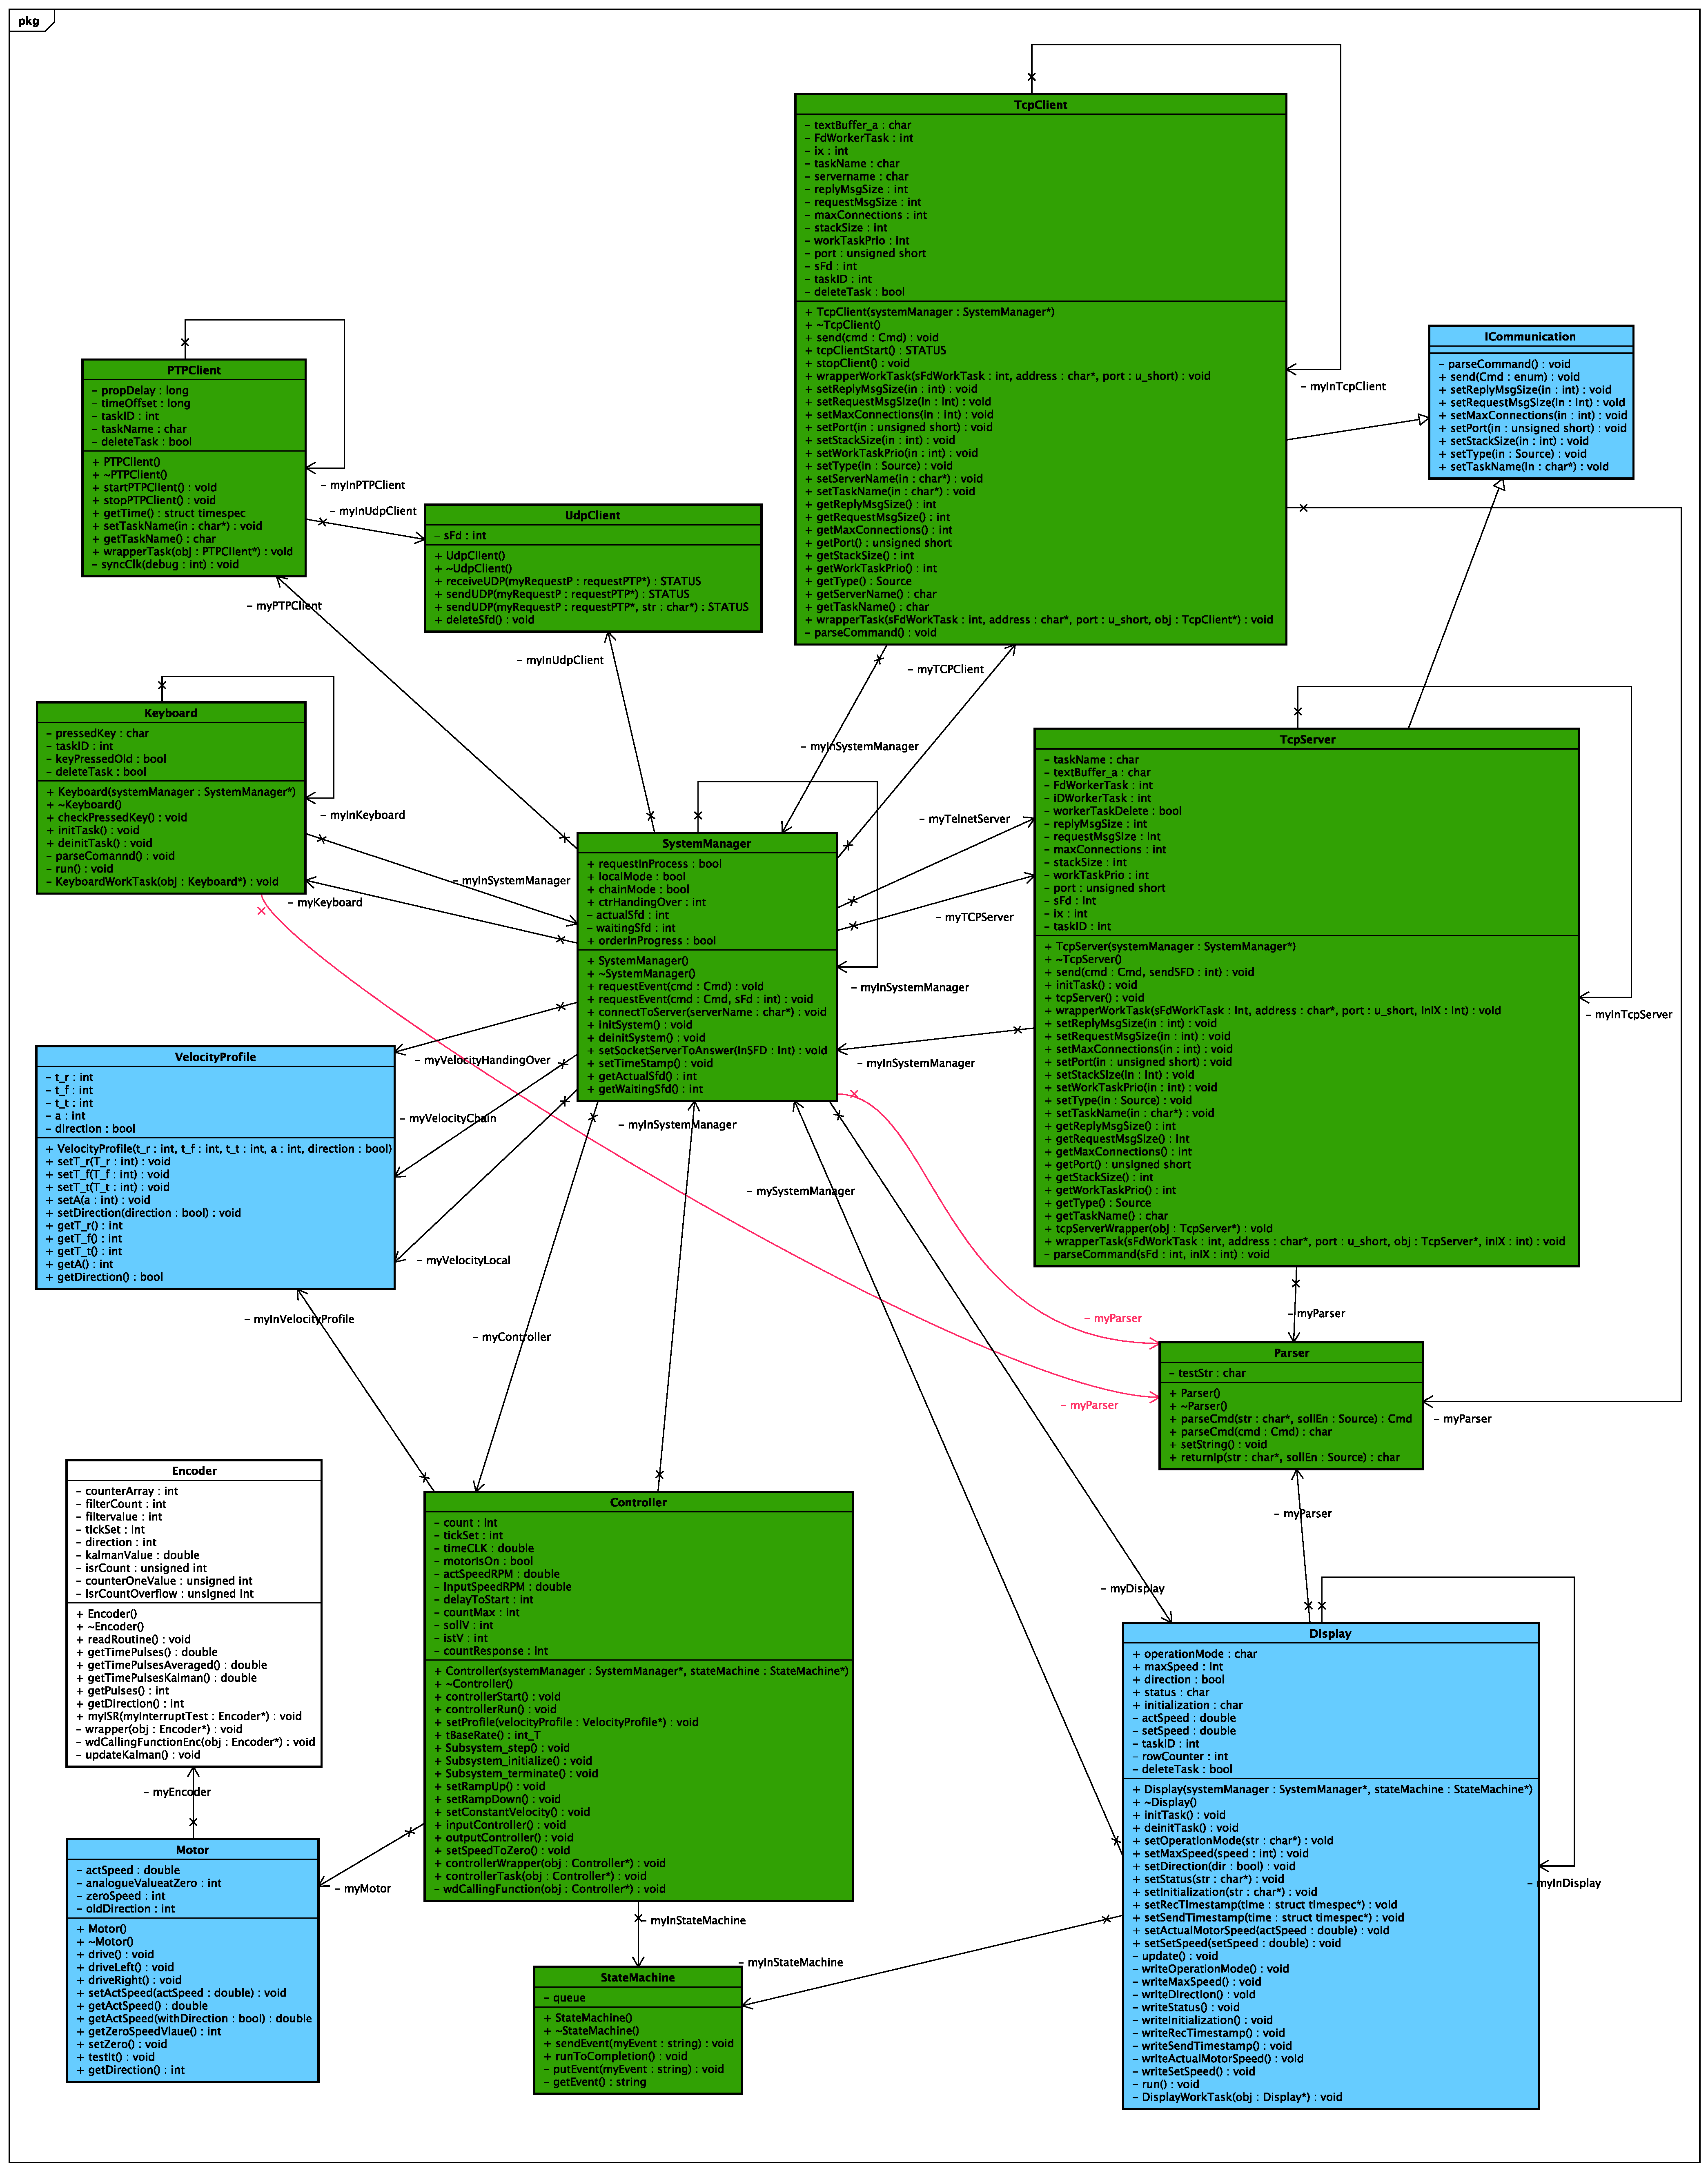
\includegraphics[width=1\textwidth]{./img/2_stat_software_strukt/ClassDiagram_implementation.pdf}
	}
	\unterschrift{Implementiertes Klassendiagramm}{Eigene Ausarbeitung}{}
	\label{fig: ClassDiagram_implementation.pdf}
\end{figure}
%
In \autoref{tab: task beschreibung} sind die Tasks, die von der Applikation gestartet werden, kurz beschrieben.
%
\begin{table}[H]
	\centering
	\noindent\adjustbox{max width=\linewidth}{
		\begin{tabular}{|c|c|p{8.5cm}|}\hline 
			&Priorität & Beschreibung \\ \hline
			tMain	&100		&	Dieser Task initialisiert alle Klassen und bleibt in der \enquote{blocking} Funktion der Statemachine stehen, d.h. er ist für die Abarbeitung der Events der Statemachine zuständig.	\\ \hline
			tBaseRate	&50		&	Der Task wird für den Regler benötigt und hat eine zyklische Periode von \(15~ms\).	\\ \hline
			tController	&150		& Ist der Task, der für den Regler benötigt wird, um ihn wieder zu beenden. \\ \hline
			tDisplay	&110		& Dieser Task beschreibt zyklisch alle \(50~ms\) das Display neu.\\ \hline
			tEncoder	&90		& Dieser Task ist für die Auswertung des Kalmanfilters zuständig und hat eine Periode von \(5~ms\).\\ \hline
			tKeyboard	&110		& Dieser Task ist für die Eingabe der Tastatur am Versuchsaufbau zuständig und arbeitet mit einer Periode von \(80~ms\).\\ \hline
			tPtpClient	&110		& Dieser Task ist für den Empfang und das Senden der \gls{ptp} Pakete zuständig und läuft azyklisch, da \enquote{blocking} Funktionen verwendet werden. \\ \hline
			tTcpServer	&101		& Dieser Task ist für den Verbindungsaufbau zu den Förderbändern und den Master zuständig und läuft azyklisch, da \enquote{blocking} Funktionen verwendet werden.\\ \hline
			FdWorkerTask\textbf{x}	&101	& Dieser Task empfängt die Daten und läuft azyklisch, da \enquote{blocking} Funktionen verwendet werden. Das \enquote{\textbf{x}} steht für einen Workertask von \(1\) bis \(10\).\\ \hline
			tTcpClient	&107		& Dieser Task empfängt die Daten und läuft azyklisch, da \enquote{blocking} Funktionen verwendet werden. \\ \hline
			tTcpTelnet	&102		& Dieser Task empfängt die Daten und läuft azyklisch, da \enquote{blocking} Funktionen verwendet werden.\\ \hline
		\end{tabular} 
	}
	\unterschrift{Beschreibung der Tasks}{Eigene Ausarbeitung}{}
	\label{tab: task beschreibung}
\end{table}
%
\end{document}
